\documentclass[12pt]{article}
\usepackage[brazilian]{babel}
\usepackage[utf8x]{inputenc}
\usepackage{amsmath}	
\usepackage{graphicx}
\usepackage{gensymb}
\usepackage[colorinlistoftodos]{todonotes}
\usepackage{listings}

\usepackage{multicol}
\usepackage{multirow}
\pagenumbering{gobble}
\usepackage{marvosym, wasysym}

\addtolength{\hoffset}{-2.25cm}
\addtolength{\textwidth}{4.5cm}
\addtolength{\voffset}{-2.5cm}
\addtolength{\textheight}{5cm}
\setlength{\parskip}{0pt}
\setlength{\parindent}{0in}

\usepackage{booktabs,array,lmodern}

\begin{document}

\title{Documentação de Projeto de um Processador de 70 instruções}

\begin{titlepage}
 
\newcommand{\HRule}{\rule{\linewidth}{0.5mm}} % Defines a new command for the horizontal lines, change thickness here

\center % Center everything on the page

\begin{figure}[!htb]
\centering
\includegraphics[width=0.2\textwidth]{Figuras/logo_ufrn.png}
\end{figure}

\textsc{\LARGE Universidade Federal do Rio Grande do Norte}\\[2cm] % Name of your university/college
\textsc{\Large ELE1717 - SISTEMAS DIGITAIS}\\[1cm] % Major heading such as course name

\HRule \\[0.6cm]
{ \huge \bfseries Datasheet do Processador}\\[0.4cm] % Title of your document
\HRule \\[1cm]

\textsc{\large Projeto e Documentação de um processador de 70 instruções}\\[3.5cm] % Minor heading such as course title
 
%----------------------------------------------------------------------------------------
%	AUTHOR SECTION
%----------------------------------------------------------------------------------------

\begin{minipage}{0.4\textwidth}
\begin{flushleft} \large
\emph{Discentes:}\\
\begin{tabbing}
Ana Karoline Pontes Machado\\
Camila Barbosa Gomes de Araújo \\
Gabriel Teixeira Vantuil\\
\end{tabbing}
\end{flushleft}
\end{minipage}
~
\begin{minipage}{0.4\textwidth}
\begin{flushright} \large
\emph{Docente:}\\
Samaherni Morais Dias \\
~
\end{flushright}
\end{minipage}\\[2cm]

\bigskip
\bigskip
\bigskip
\bigskip
\bigskip
\bigskip

{\large \today}\\[2cm] % Date, change the \today to a set date if you want to be precise

\end{titlepage}

Esse documento descreve e documenta o projeto de um processador de 8 bits e 69 instruções para a disciplina de Sistemas Digitais (ELE1717). O processador foi implementado em VHDL, simulado com o auxílio do Quartus e também executado na FPGA Cyclone II. 

\bigskip

O Processador implementado possui arquitetura Von-Neumann (RAM 256x8-Bits), com 4 registradores de uso geral (A,B,C,D) de 8 bits cada, com um ponteiro para pilha (SP) de 8 Bits (na configuração SP-1 com SP máximo no endereço 231), com 2 bits de sinalização Z (True se o resultado da ULA for zero) e C (True se a ULA apresentar um carry de saída), com 24 posições de I/O representadas pelos endereços de 232 até 255 da memória RAM. 

\bigskip

Nesse documento será explicado:

\begin{itemize}
\item A escolha dos opcodes para as 69 instruções
\item A descrição dos componentes do Data Path
\item A descrição dos componentes do Controlador
\item A listagem e especificações dos sinais de controle
\item Máquina de Estados
\item Desenho completo da modelagem do Processador
\end{itemize}

\section{Visão geral do Processador}
Dividimos o processador em data path e em controller. O data path contém a ULA e o banco de registradores. Já o controle é onde se executa a máquina de estados e onde acontece a manipulação dos opcodes, onde se localiza o ponteiro para pilha e o contador do programa. Abaixo segue um esquemático simplificado do processador desenvolvido.

\begin{figure}[!htb]
\centering
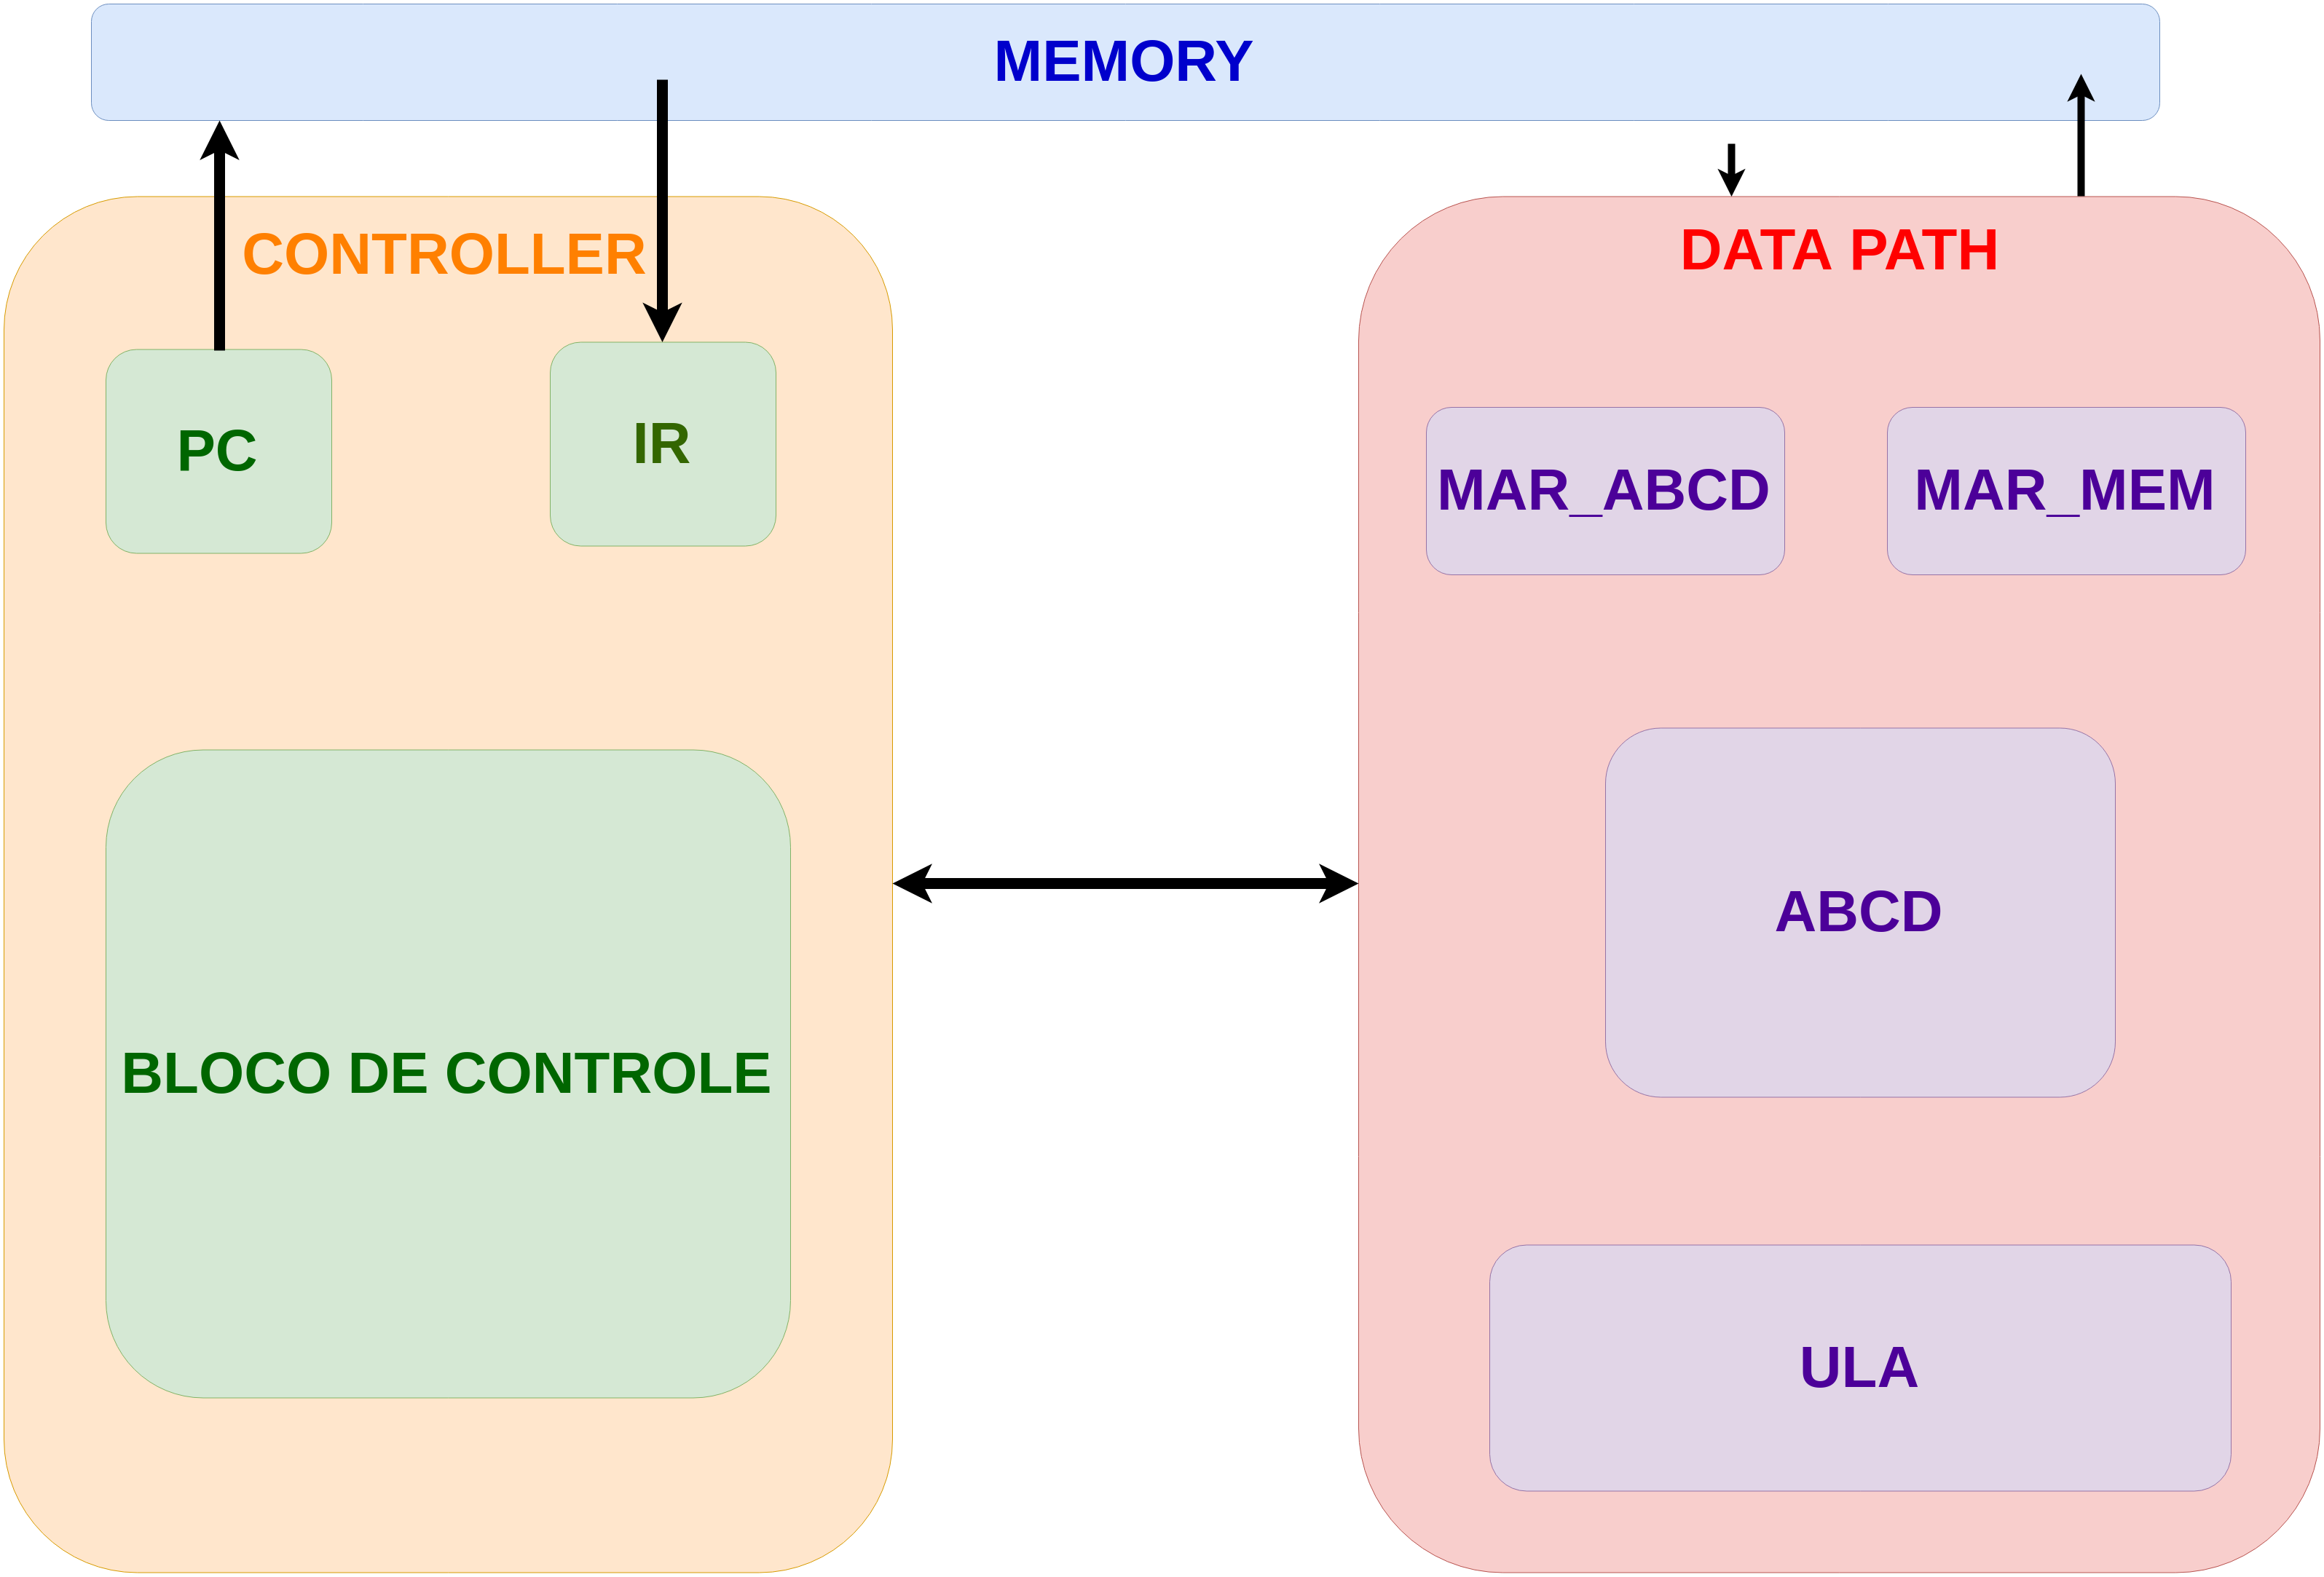
\includegraphics[width=0.7\textwidth]{Figuras/geral.png}
\end{figure}

\section{Escolha de Opcodes}
A escolha dos opcodes foi estratégica para tentar diminuir o máximo possível o número de estados distintos na MDE. Logo, instruções com a mesma sequência de estados, foram padronizadas para facilitar a implementação. A tabela de opcodes está anexada a esse documento.

%https://www.tablesgenerator.com/latex_tables
\begin{table}[!htbp]
\centering
\begin{tabular}{|c|c|c|c|c}
\hline
\multicolumn{5}{|c|}{TABELA DE OPCODES}                                                                                                                 \\ \hline
opcode(7)           & opcode(6 downto 3)      &                      & opcode(2 downto 0)     & \multicolumn{1}{c|}{Parâmetros}                                   \\ \hline
\multirow{16}{*}{0} & "0000"                  & ADD                  & \multirow{2}{*}{"000"} & \multicolumn{1}{c|}{\multirow{2}{*}{reg, regX}}         \\ \cline{2-3}
                    & "0001"                  & SUB                  &                        & \multicolumn{1}{c|}{}                                   \\ \cline{2-5} 
                    & "0010"                  & AND                  & \multirow{2}{*}{"001"} & \multicolumn{1}{c|}{\multirow{2}{*}{reg, {[}regX{]}}}   \\ \cline{2-3}
                    & "0011"                  & OR                   &                        & \multicolumn{1}{c|}{}                                   \\ \cline{2-5} 
                    & "0100"                  & XOR                  & \multirow{2}{*}{"010"} & \multicolumn{1}{c|}{\multirow{2}{*}{reg,{[}address{]}}} \\ \cline{2-3}
                    & "0101"                  & SHL                  &                        & \multicolumn{1}{c|}{}                                   \\ \cline{2-5} 
                    & "0110"                  & SHR                  & \multirow{2}{*}{"011"} & \multicolumn{1}{c|}{\multirow{2}{*}{reg, constant}}     \\ \cline{2-3}
                    & "0111"                  & CMP                  &                        & \multicolumn{1}{c|}{}                                   \\ \cline{2-5} 
                    & "1000"                  & PUSH                 & \multirow{2}{*}{"100"} & \multicolumn{1}{c|}{\multirow{2}{*}{reg}}               \\ \cline{2-3}
                    & "1001"                  & POP                  &                        & \multicolumn{1}{c|}{}                                   \\ \cline{2-5} 
                    & "1010"                  & MUL                  & \multirow{2}{*}{"101"} & \multicolumn{1}{c|}{\multirow{2}{*}{{[}reg{]}}}         \\ \cline{2-3}
                    & "1011"                  & CALL                 &                        & \multicolumn{1}{c|}{}                                   \\ \cline{2-5} 
                    & "1100"                  & INC                  & \multirow{2}{*}{"110"} & \multicolumn{1}{c|}{\multirow{2}{*}{address}}           \\ \cline{2-3}
                    & "1101"                  & DEC                  &                        & \multicolumn{1}{c|}{}                                   \\ \cline{2-5} 
                    & "1110"                  & NOT                  & \multirow{2}{*}{"111"} & \multicolumn{1}{c|}{\multirow{2}{*}{constant}}          \\ \cline{2-3}
                    & "1111"                  & JMP                  &                        & \multicolumn{1}{c|}{}                                   \\ \hline
\multirow{23}{*}{1} & \multirow{7}{*}{"0000"} & \multirow{7}{*}{MOV} & "000"                  & \multicolumn{1}{c|}{reg, regX}                          \\ \cline{4-5} 
                    &                         &                      & "001"                  & \multicolumn{1}{c|}{reg, {[}regX{]}}                    \\ \cline{4-5} 
                    &                         &                      & "010"                  & \multicolumn{1}{c|}{reg, {[}address{]}}                 \\ \cline{4-5} 
                    &                         &                      & "011"                  & \multicolumn{1}{c|}{reg, constant}                      \\ \cline{4-5} 
                    &                         &                      & "100"                  & \multicolumn{1}{c|}{{[}reg{]}, regX}                    \\ \cline{4-5} 
                    &                         &                      & "101"                  & \multicolumn{1}{c|}{{[}address{]}, reg}                 \\ \cline{4-5} 
                    &                         &                      & "110"                  & \multicolumn{1}{c|}{{[}address{]}, constante}           \\ \cline{2-5} 
                    & "0001"                  & JC                   & \multirow{14}{*}{X}    & \multicolumn{1}{c|}{}                                   \\ \cline{2-3} \cline{5-5} 
                    & "0010"                  & JNC                  &                        & \multicolumn{1}{c|}{}                                   \\ \cline{2-3} \cline{5-5} 
                    & "0011"                  & JZ                   &                        & \multicolumn{1}{c|}{}                                   \\ \cline{2-3} \cline{5-5} 
                    & "0100"                  & JNZ                  &                        & \multicolumn{1}{c|}{}                                   \\ \cline{2-3} \cline{5-5} 
                    & "0101"                  & JA                   &                        & \multicolumn{1}{c|}{}                                   \\ \cline{2-3} \cline{5-5} 
                    & "0110"                  & JNBE                 &                        & \multicolumn{1}{c|}{}                                   \\ \cline{2-3} \cline{5-5} 
                    & "0111"                  & JAE                  &                        & \multicolumn{1}{c|}{}                                   \\ \cline{2-3} \cline{5-5} 
                    & "1000"                  & JNB                  &                        & \multicolumn{1}{c|}{}                                   \\ \cline{2-3} \cline{5-5} 
                    & "1001"                  & JB                   &                        & \multicolumn{1}{c|}{}                                   \\ \cline{2-3} \cline{5-5} 
                    & "1010"                  & JNAE                 &                        & \multicolumn{1}{c|}{}                                   \\ \cline{2-3} \cline{5-5} 
                    & "1011"                  & JBE                  &                        & \multicolumn{1}{c|}{}                                   \\ \cline{2-3} \cline{5-5} 
                    & "1100"                  & JNA                  &                        & \multicolumn{1}{c|}{}                                   \\ \cline{2-3} \cline{5-5} 
                    & "1101"                  & JE                   &                        & \multicolumn{1}{c|}{}                                   \\ \cline{2-3} \cline{5-5} 
                    & "1110"                  & JNE                  &                        & \multicolumn{1}{c|}{}                                   \\ \cline{2-5} 
                    & \multirow{2}{*}{"1111"} & RET                  & "000"                  & \multicolumn{1}{c|}{}                                   \\ \cline{3-5} 
                    &                         & HLT                  & "111"                  &                                                         \\ \cline{1-4}
\end{tabular}
\end{table}

\section{Data Path}
Nosso data path possui 2 registradores auxiliares, o  MAR\_MEM e o MAR\_ABCD. Além disso, possui um banco de registradores, o ABCD, com apenas 4 registradores. Tal banco possui apenas 1 entrada de endereço e uma saída apenas. Todavia, existe uma saída permanente do registrador com o valor do registrador A. Tal saída é usada somente na multiplicação.

\begin{figure}[!htb]
\centering
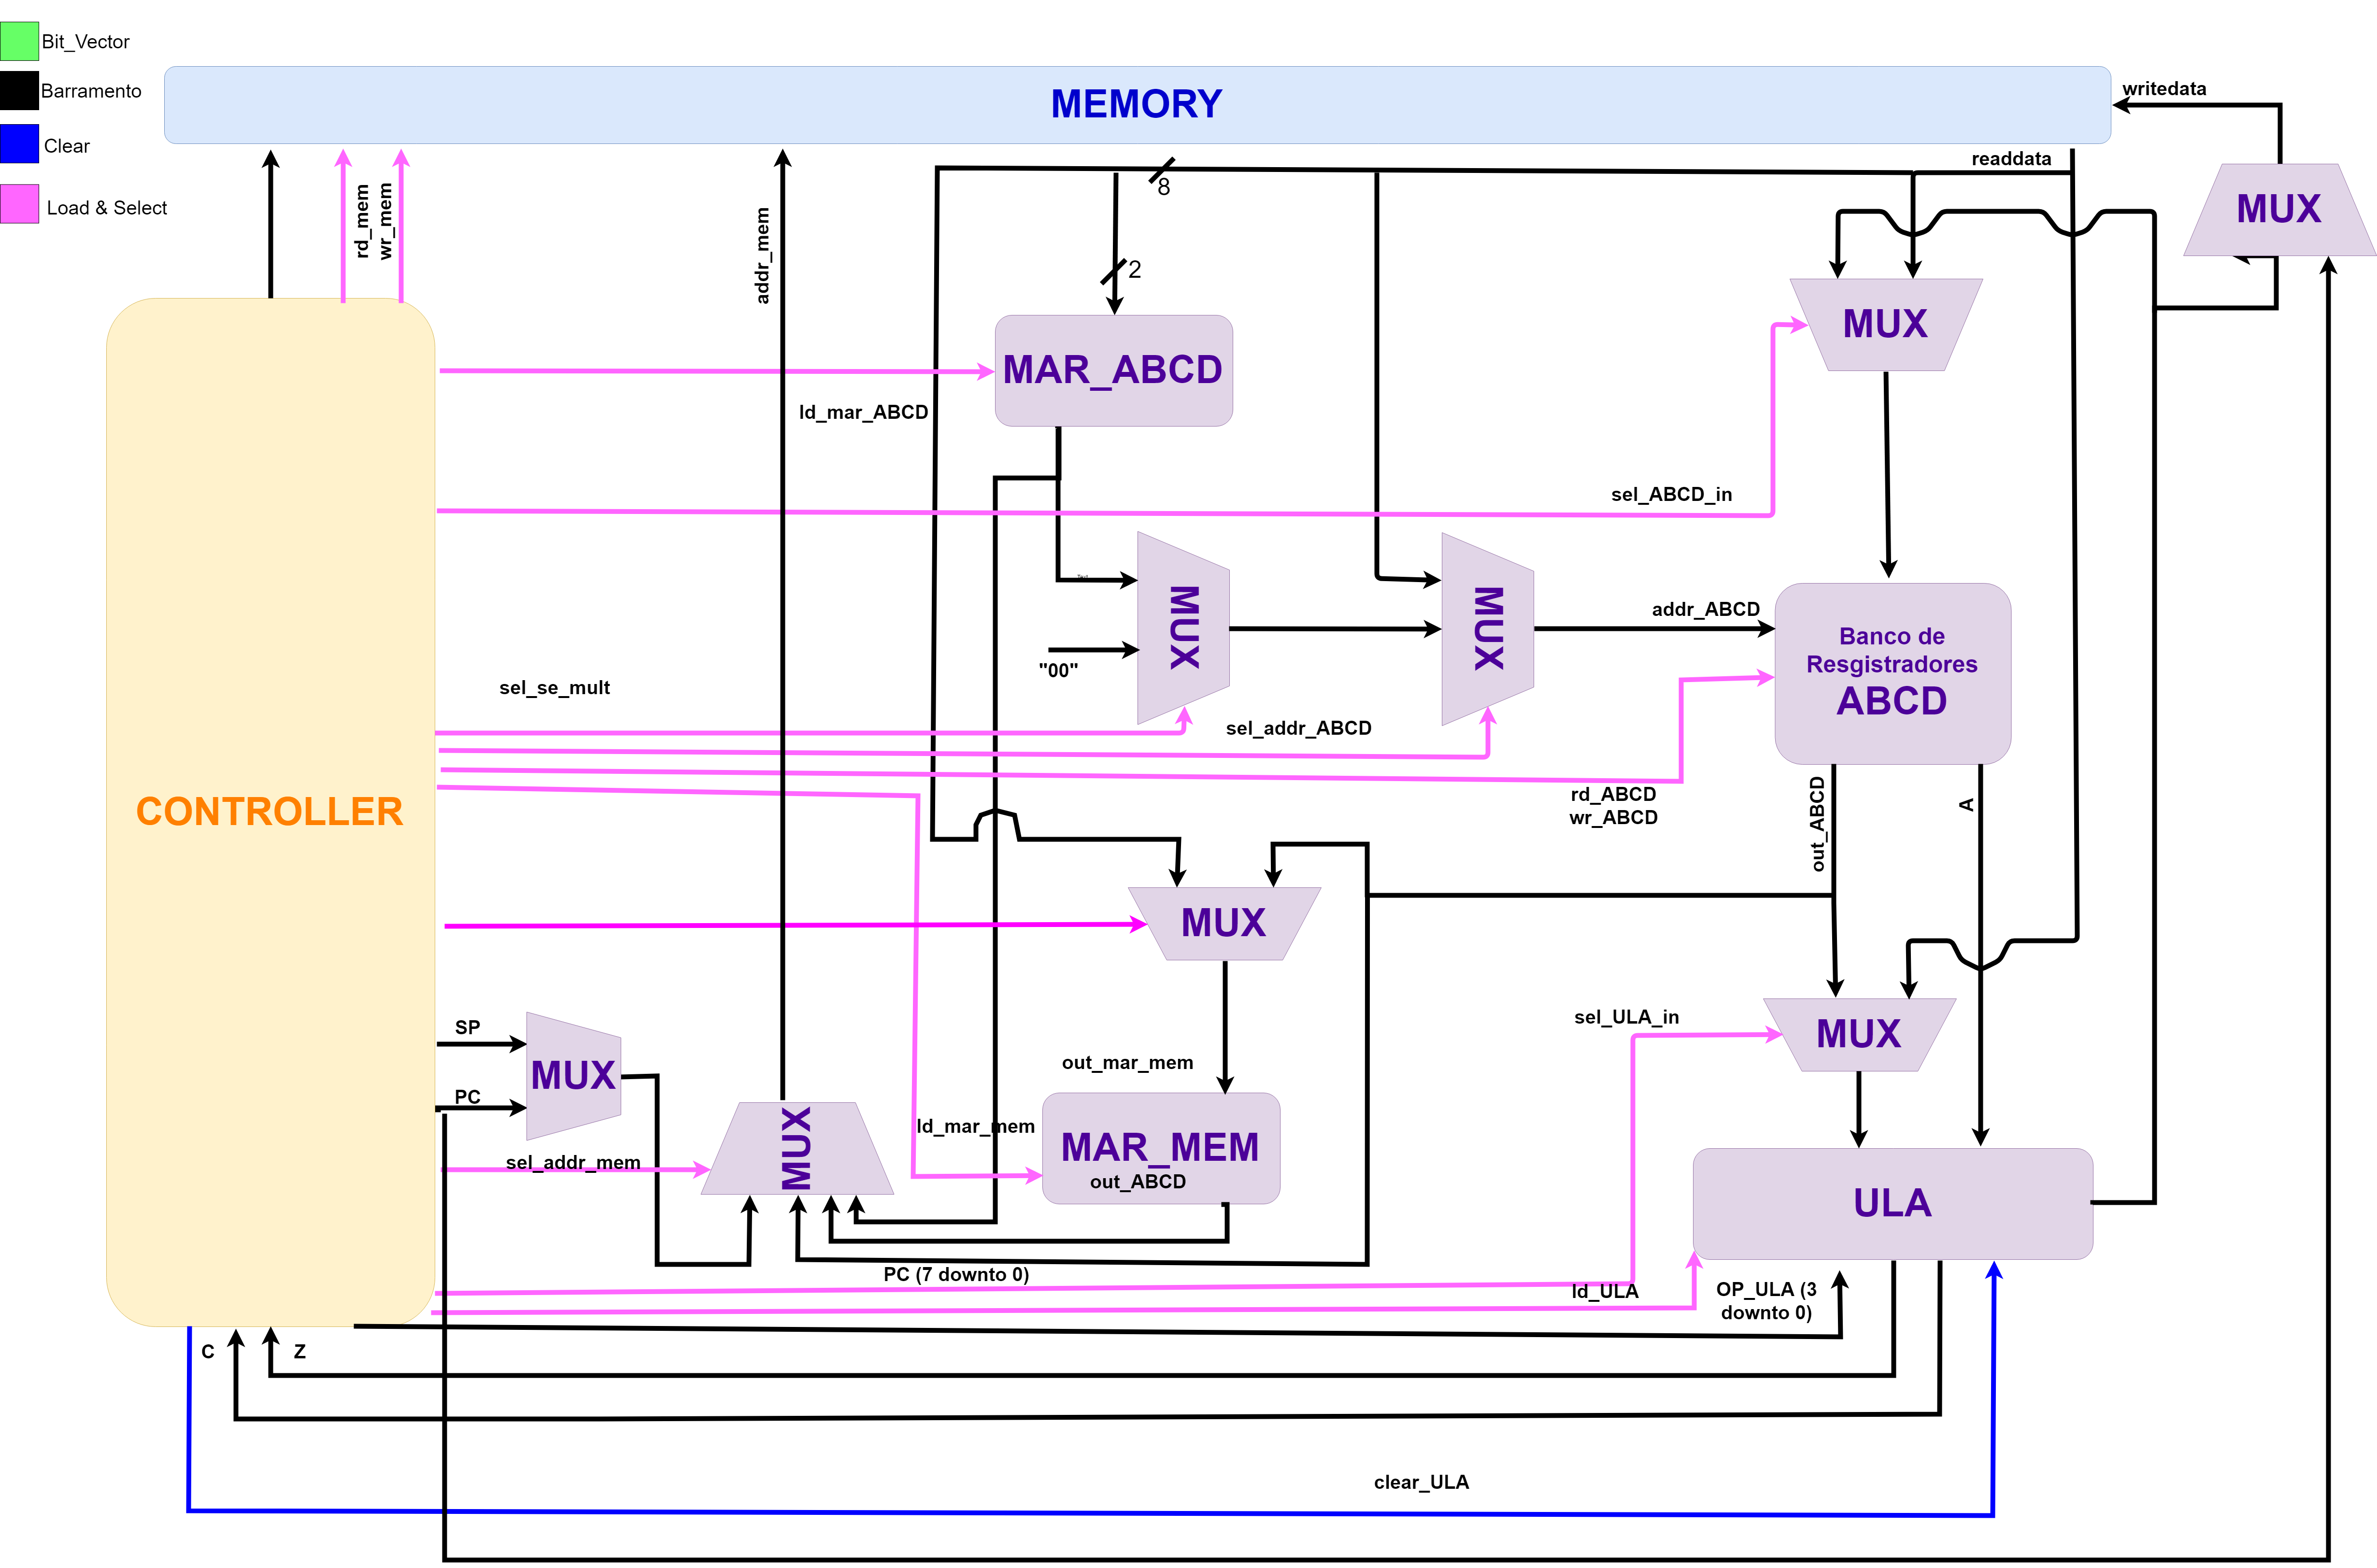
\includegraphics[width=0.7\textwidth]{datapath.png}
\end{figure}

\section{Controlador}

\begin{figure}[!htb]
\centering
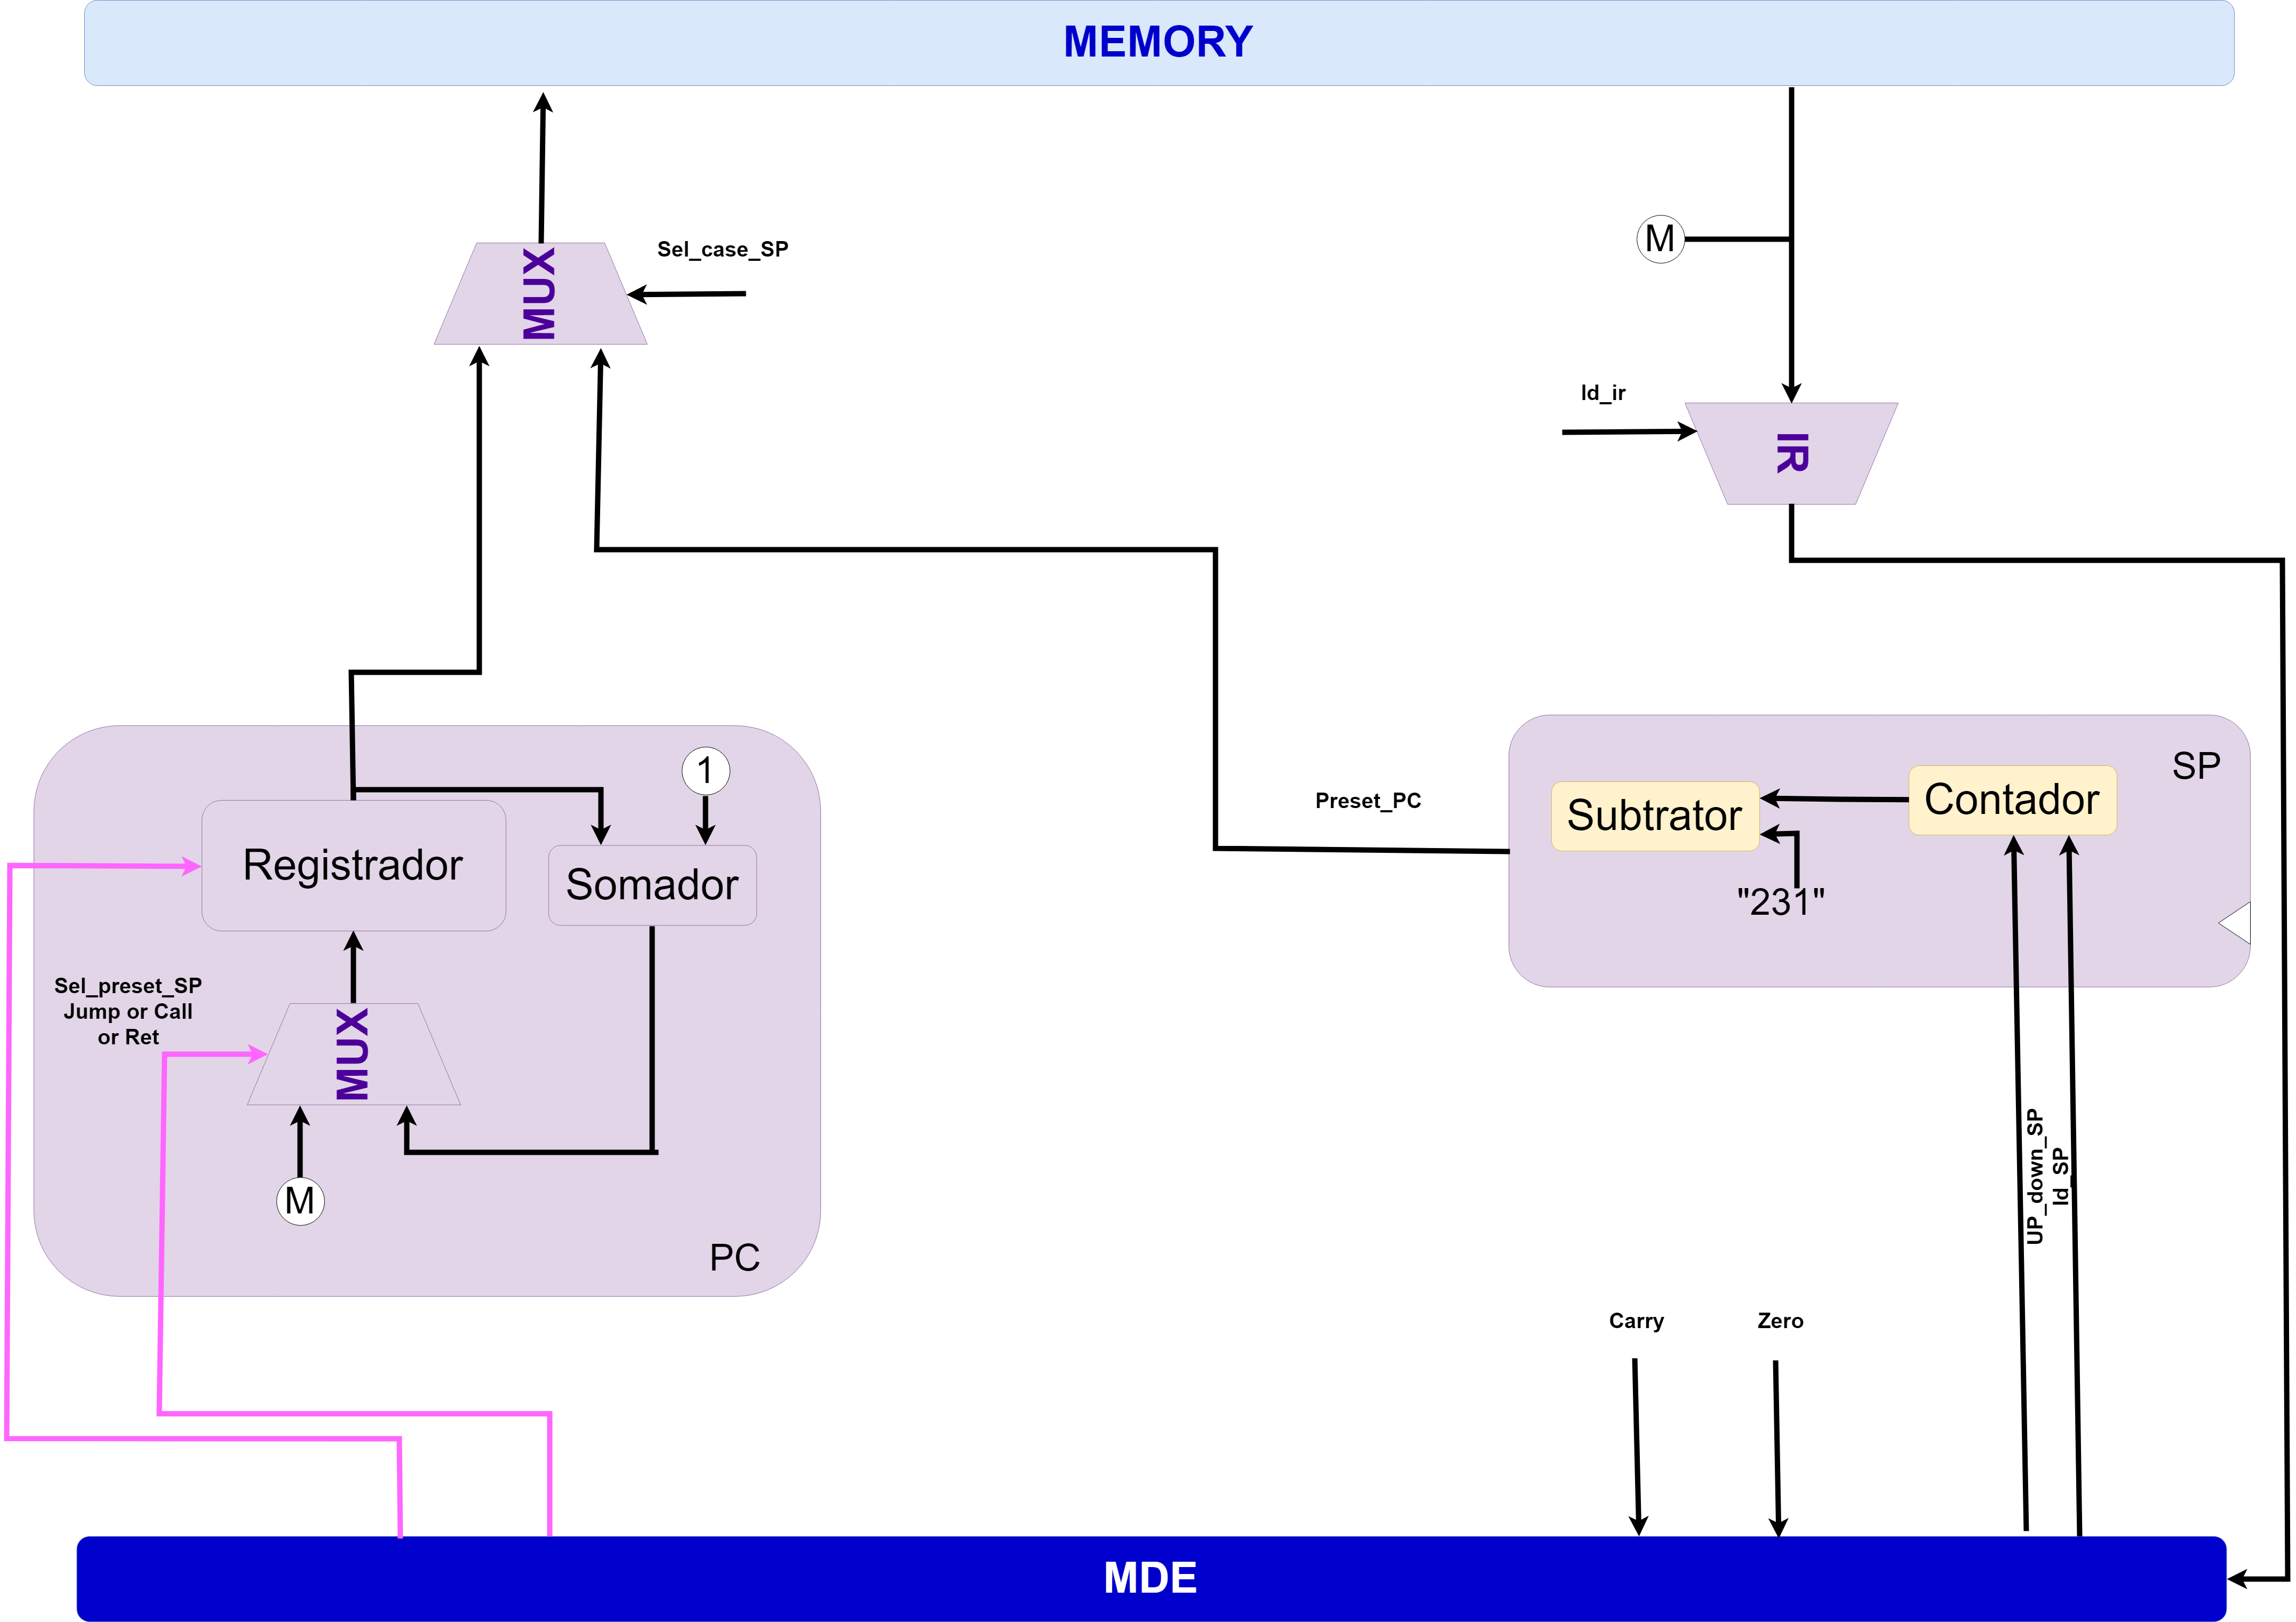
\includegraphics[width=0.7\textwidth]{controller.png}
\end{figure}


\section{Sinais de Controle}
Podemos classificar os sinais que saem da máquina de estados em dois grupos, os que irão controlar o fluxo de ações do data path e os que vão controlar o fluxo de ações do controlador. Abaixo seguem os sinais saídos da máquina de estados para o data path:

\begin{itemize}
\item Sel\_mar\_mem: bit de seleção para o mux da entrada do registrador MAR\_mem. '0' = saída da memória RAM; '1' = saída do banco de registradores;
\item Ld\_mar\_mem: load do registrador MAR\_mem
\item Sel\_se\_mult: bit de seleção do mux que seleciona o registrador A para entrada de endereço do banco de registradores (usado para o caso da operação MUL). '0' = caso não seja operação de multiplicação; '1' = caso seja multiplicação;
\item Wr\_ABCD: bit de controle que escreve no banco de registradores ABCD
\item Ld\_mar\_ABCD: load do registrador MAR\_ABCD
\item Sel\_addr\_ABCD: bit de seleção para o endereço do banco de registradores ABCD. Seleciona entre a saída do mux "se\_mult" e a saída da RAM. "00" = saída do mux PC ou SP; "01" = saída do registrador MAR\_mem; "10" = saída do banco de registradores ABCD; "11" = saída do registrador MAR\_ABCD;
\item Sel\_addr\_mem: bits de seleção da entrada de endereço na memória RAM. . "00" = PC ou SP; "01" = saída do MAR\_mem; "10" = ; "11" = saída ;
\item Wr\_mem: bit de controle que escreve na memória RAM
\item Sel\_mem\_in: bit de seleção do mux da entrada de dados na memória, seleciona entre a saída da ULA e o PC. '0' = saída da ULA; '1' = PC;
\item Sel\_ABCD\_in: bit de seleção do mux da entrada de dados no banco de registradores, seleciona entre a saída da ULA e a saída da memória. '0' = saída da memória; '1' = saída da memória;
\item Sel\_ULA\_in: bit de seleção do mux da entrada da ULA, seleciona entre a saída da memória e a saída do banco de registradores. '0' = saída do banco de registradores; '1' = saída da memória;
\item Ld\_ULA: load da ULA
\item Clr\_ULA: clear da ULA
\end{itemize}

Os sinais que vão para o controlador são, em sua maioria, para controlar o apontador para a pilha (SP) e para o contador do programa (PC). Abaixo segue a lista desses sinais e suas respectivas especificações:

\begin{itemize}
\item Sel\_case\_SP: bit de seleção do mux para seleção de addr na memória, caso '1', a saída é o SP, caso '0', a saída é o PC
\item Ld\_IR: load do IR
\item Ld\_PC: load do PC
\item Ld\_SP: load do SP
\item Up\_down\_SP: Seleciona se o contador presente na estrutura do SP irá contar up ou down. UP='1', DOWN='0';
\item Sel\_preset\_PC: Seleciona o mux de entrada para o preset do registrador PC. Caso '1', o preset do PC é ativado (jmp ou instruções de pilha), caso '0', não há preset;
\end{itemize}

\section{Máquina de Estados}
A máquina de estados é relativamente complexa devido ao extenso número de instruções. Para cada estado, dependendo do opcode, o valor de várias variáveis de controle serão diferentes. Segue a tabela com tais variáveis e em que estado elas mudam. É válido lembrar que o valor padrão de tais variáveis sempre será '0', logo, só serão apresentadas na tabela os valores de tais mudanças.

\begin{figure}[!htbp]
\centering
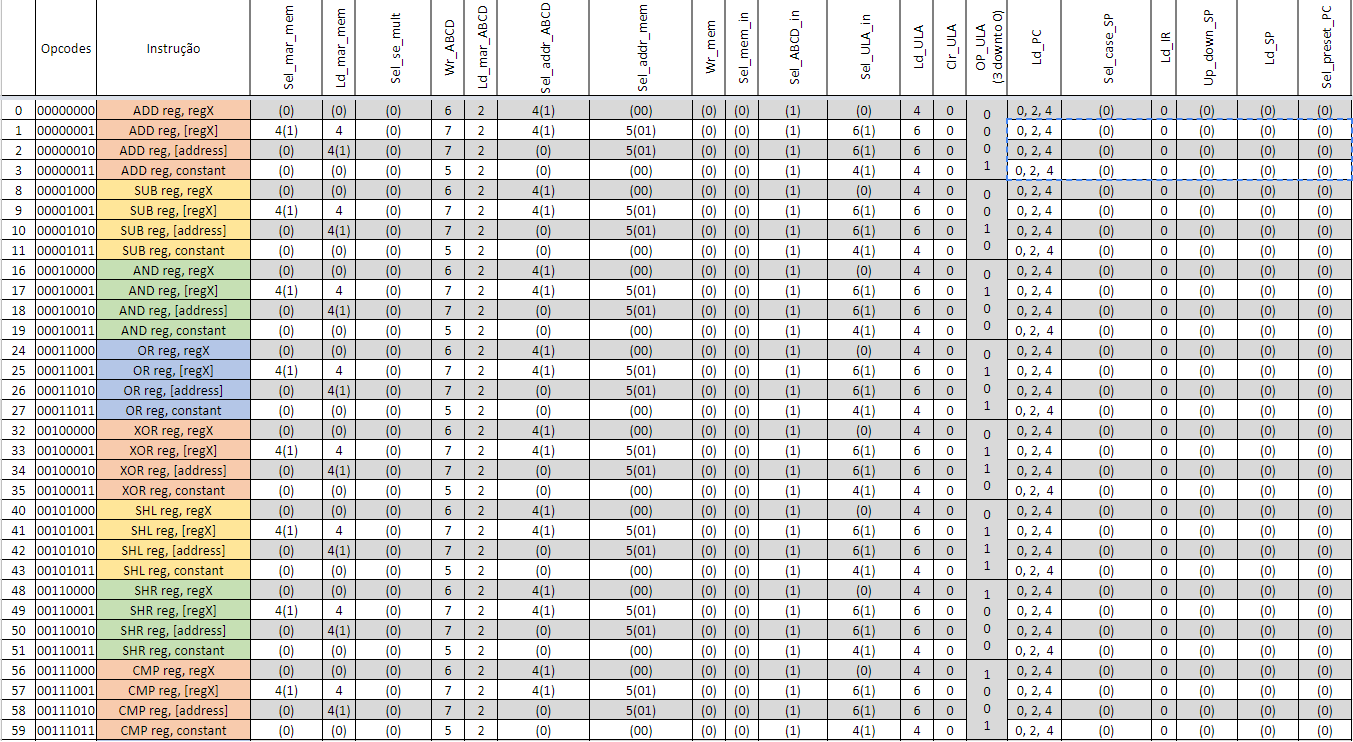
\includegraphics[width=1\textwidth]{Figuras/mde1.png}
\end{figure}

\begin{figure}[!htbp]
\centering
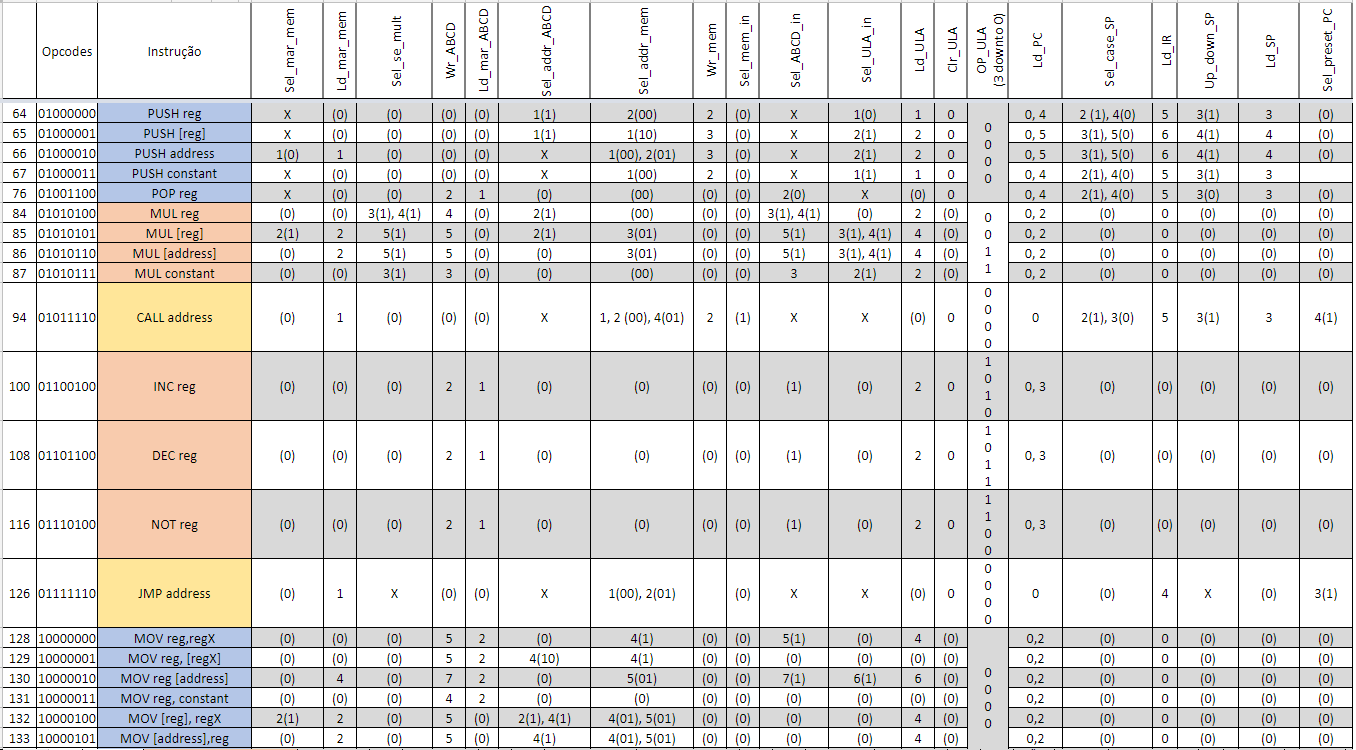
\includegraphics[width=1\textwidth]{Figuras/mde2.png}
\end{figure}

\begin{figure}[!htbp]
\centering
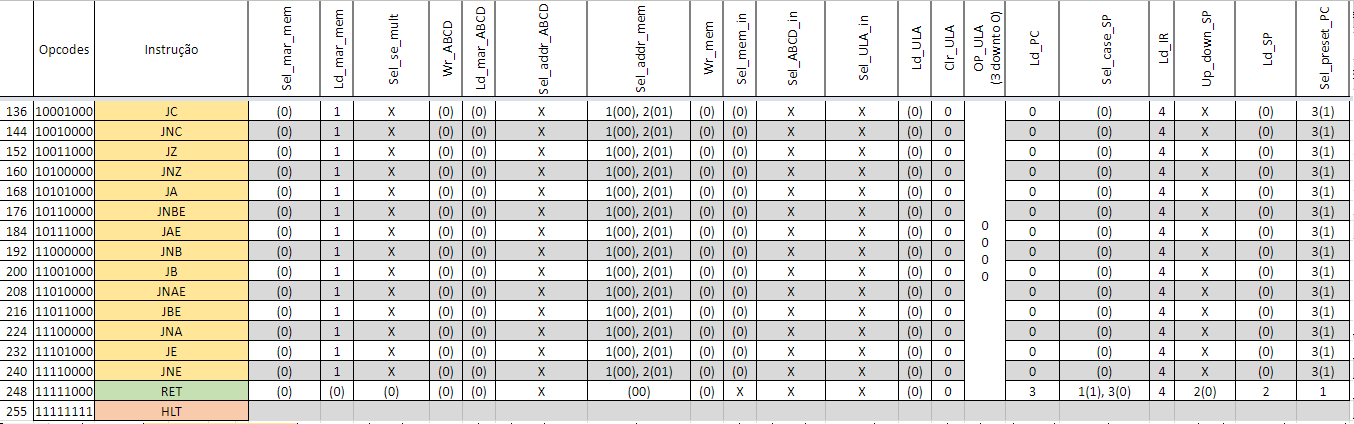
\includegraphics[width=1\textwidth]{Figuras/mde3.png}
\end{figure}



\end{document}



